\documentclass[12pt]{article}
\usepackage{graphicx} % Required for inserting images
\usepackage{amsmath,amssymb,amsthm,amsfonts}
\usepackage{xcolor}
\usepackage{tasks}
%\usepackage{enumitem}
\usepackage[margin=1cm]{geometry}
\usepackage{tkz-euclide}
\usepackage{multicol}

\usepackage[utf8]{inputenc}
\usepackage[T1]{fontenc}
\usepackage{amsmath}
\usepackage{amsfonts}
\usepackage{amssymb}
\usepackage[version=4]{mhchem}
\usepackage{stmaryrd}
\usepackage{enumerate}
\usepackage{multicol}
\usepackage{xcolor}
\usepackage{graphicx}
\usepackage{ulem}
\usepackage{cancel}
\usepackage{tikz}
\usepackage{tkz-euclide}
\usepackage[finnish]{babel}

%\usepackage[style=alphabetic,]{biblatex}

%\usepackage[margin=2cm]{geometry}

\newcommand{\brac}[1]{\left(#1\right)}
\newcommand{\sqbrac}[1]{\left[#1\right]}
\newcommand{\set}[1]{\left\{#1\right\}}

\newcommand{\dd}[0]{\mathrm{d}}
\newcommand{\dx}[0]{\mathrm{d}x}

\newcommand{\hatu}{\hat{u}}
\newcommand{\hatv}{\hat{v}}
\newcommand{\hatw}{\hat{w}}
\newcommand{\hatn}{\hat{n}}

\newcommand{\vu}{\overline{u}}
\newcommand{\vv}{\overline{v}}
\newcommand{\vw}{\overline{w}}
\newcommand{\vp}{\overline{p}}
\newcommand{\vn}{\overline{n}}

\newcommand{\va}{\overline{a}}
\newcommand{\vb}{\overline{b}}
\newcommand{\vc}{\overline{c}}
\newcommand{\vd}{\overline{d}}


\newcommand{\vi}{\hat{\imath}}
\newcommand{\vj}{\hat{\jmath}}
\newcommand{\vk}{\hat{k}}

\newcommand{\ratkaisu}[1]{\hfill{\color{blue}\quad\textrm{Ratkaisu: } #1}}

\newcommand{\ratkaisuu}[1]{{\color{blue}\textrm{Ratkaisu: } #1}}

\newcommand{\kaava}[1]{{\color{green!50!black}#1}}

%\renewcommand{\ratkaisu}[1]{}
%\renewcommand{\ratkaisuu}[1]{}
%\renewcommand{\kaava}[1]{}

\newcommand{\vihje}[1]{{\color{red}Vihje. #1}}
\newcommand{\extra}[0]{\textbf{Extra.}~}

\title{OAMK}
\author{Juha-Matti Huusko}
\date{August 2023}

\renewcommand{\ratkaisu}[1]{{\color{blue}\quad\textrm{Ratkaisu: } #1}}

\renewcommand{\ratkaisu}[1]{}

\begin{document}
\thispagestyle{empty}

\section*{Koe 13.9.2024}
\subsubsection*{Matematiikan perusteet tietotekniikassa 1, IN00EH18-3002}

\begin{enumerate}
%\setlength{\itemsep}{40pt}
\item Sievennä lauseke
%$$\brac{\frac23+\frac34}\bigg/\brac{6-\frac13}$$\ratkaisu{1/4} %ma
    $$\brac{\frac32+\frac25}\bigg/\brac{3-\frac16}$$\ratkaisu{1/2} %ti
    %$$\brac{\frac14-\frac13}\bigg/\brac{2-\frac16}\ratkaisu{-1/22}$$\ratkaisu{-1/22}
muotoon $\frac{p}{q}$, missä $p$ ja $q$ ovat kokonaislukuja.

\item Avaa sulut
%$$(2x-3)^2-2(1-6x).$$\ratkaisu{$4x^2+7$} %ma
$$(4x-3)^2-3(5-2x).$$\ratkaisu{$16x^2$} %ti

%$$(2x+3)^2-x(8+4x).\ratkaisu{4x+9}$$

\item Ratkaise toisen asteen yhtälö
%$$x^2-5x+4=0.$$\ratkaisu{$x=1,x=4$}
$$x^2-7x+10=0$$\ratkaisu{$x=-1,x=2$} %ti

\item Ratkaise yhtälöparista
%$$
%\begin{cases}
%5x+y&=6\\
%-4x+y&=-6
%\end{cases}\ratkaisu{$x=4/3, y=-2/3$}
%$$
$$\begin{cases}
5x+2y&=6\\
2x-y&=3
\end{cases}\ratkaisu{$x=2/3, y=-1/3$}
$$
tuntemattomat $x$ ja $y$.

\def\a{2}\def\b{7}\def\c{3}\def\d{2} %ma
%\def\a{3}\def\b{4}\def\c{5}\def\d{2} %ti
%\def\a{7}\def\b{2}\def\c{4}\def\d{5} %aiempi


\item Ratkaise $x$ yhtälöstä
$$
\a^{\b x}=\c^{x+\d}.
$$
\ratkaisu{$x=\frac{\d \ln(\c)}{\b \ln(\a)-\ln(\c)}$}

\item Ratkaise $x$ yhtälöstä

%$$2\ln(5x)-\ln(x)=\ln(4x+7)$$\ratkaisu{$x=1/24$}
$$2\ln(5x^3)-5\ln(x)=\ln(7x+3).$$\ratkaisu{$x=1/6$} %ti

%$$3\ln(2x)-2\ln(x)=\ln(x+1).\ratkaisu{x=\frac{1}{7}}$$

\item Selvitä oheisessa kolmiossa kateettien $a$ ja $b$ pituudet ja kulman $\beta$ suuruus.

%31 ja %21
\def\kulma{41}
\def\hypotenuusa{7}
\def\tkulma{49}
\pgfmathsetmacro{\vastainen}{int(10*\hypotenuusa*sin(\kulma))/10}
\pgfmathsetmacro{\viereinen}{int(10*\hypotenuusa*cos(\kulma))/10}


%tekstit
\def\hypotenuusaNimi{\hypotenuusa}
\def\viereinenNimi{\viereinen}
\def\vastainenNimi{\vastainen}

\def\kulmaNimi{\kulma^\circ}
\def\tkulmaNimi{\tkulma^\circ}

%\def\hypotenuusaNimi{c}
\def\viereinenNimi{b}
\def\vastainenNimi{a}

%\def\kulmaNimi{\alpha}
\def\tkulmaNimi{\beta}

%\pgfmathparse{int(90-\kulma)}\pgfmathresult
\begin{tikzpicture}
\draw (0,0) coordinate (o);
\draw (1,0) coordinate (u);
\draw (0,1) coordinate (v);
\draw (\kulma:\hypotenuusa) coordinate (p);
\draw (u-|p) coordinate (pd);
\tkzMarkAngle(pd,o,p);
\tkzLabelAngle[pos=1.5](pd,o,p){$\kulmaNimi$};
\tkzMarkAngle(o,p,pd);
\tkzLabelAngle[pos=1.5](o,p,pd){$\tkulmaNimi$};
\tkzMarkRightAngle(o,pd,p);
\draw (o)--(pd) node[midway, below]{$\viereinenNimi$};
\draw (pd)--(p) node[midway,right]{$\vastainenNimi$};
\draw (o)--(p) node[midway,above]{$\hypotenuusaNimi$};
\end{tikzpicture}

\end{enumerate}

\section*{Kaavoja}

Murtoluvut
$$
\frac{a}{b}+\frac{c}{d}=\frac{ad}{bd}+\frac{bc}{bd}
=\frac{ad+bc}{bd},\quad 
\frac{a}{b}\cdot\frac{c}{d}=\frac{ac}{bd},\quad
\frac{a}{b}\bigg/\frac{c}{d}=\frac{a}{b}\cdot\frac{d}{c}=\frac{ad}{bc}
$$
Potenssit
$$
a^ba^c=a^{b+c},\quad 
\frac{a^b}{a^c}=a^{b-c},\quad 
(a^b)^c=a^{bc},\quad 
(ab)^c=a^ba^c,\quad 
\brac{\frac{a}{b}}^c=\frac{a^b}{b^c}
$$


Juuret
$$
(a^b)^{\frac{1}{b}}=a^{b\cdot \frac{1}{b}}=a^1=a,\quad\textrm{jos}\quad a>0,\quad 
\sqrt{a}=a^{\frac{1}{2}},\quad \sqrt[3]{a}=a^{\frac{1}{3}}
$$
Ensimmäisen asteen yhtälö
$$
ax=b\quad\Leftrightarrow\quad x=\frac{b}{a}
$$
Toisen asteen yhtälö
$$
ax^2+bx+c=0\quad\Leftrightarrow\quad x=\frac{-b\pm\sqrt{b^2-4ac}}{2a}
$$
Yhtälöpari
$$
\begin{cases}
ax+by&=U\\
cx+dy&=V
\end{cases}\quad\Rightarrow
\begin{cases}
acx+bcy&=cU\\
-acx+-ady&=-aV
\end{cases}\Rightarrow\ldots
$$

$$
\begin{cases}
ax+by&=U\\
cx+dy&=V
\end{cases}\quad\Rightarrow
y=\frac{U-ax}{b}\quad\Rightarrow
cx+d\frac{U-ax}{b}=V\Rightarrow\ldots
$$

$$
\begin{cases}
ax+by&=U\\
cx+dy&=V
\end{cases}\quad\Rightarrow
\begin{cases}
x&=\frac{Ud-bV}{ad-bc}\\
y&=\frac{aV-Uc}{ad-bc}
\end{cases}
$$
Funktio $f(x)$ ja käänteisfunktio $g(x)=f^{-1}(x)$
$$
f(g(x))=x,\quad
g(f(x))=x
$$
Logaritmit
$$
\ln(ab)=\ln(a)+\ln(b),\quad
\ln(\frac{a}{b})=\ln(a)-\ln(b),\quad
\ln(a^b)=b\ln(a)
$$


\begin{equation*}
\begin{split}
\log_a(x)=y\quad&\Leftrightarrow\quad a^y=x
\end{split}
\end{equation*}


$$
\log_a(1)=0,\quad
\log_a(a)=1,\quad
\log_a(a^x)=x,\quad
a^{\log_a(x)}=x
$$

\begin{equation*}
\begin{split}
\log_a(b^c)&=c\log_a(b)\\
\log_a(xy)&=\log_a(x)+\log_a(y)\\
\log_a\left(\frac{x}{y}\right)
&=\log_a(x)-\log_a(y)\\
\log_a(x)&=\frac{\log_b(x)}{\log_b(a)}
\end{split}
\end{equation*}

$$
\textrm{lb}(x)=\log_2(x),\quad
\lg(x)=\log_{10}(x),\quad
\ln(x)=\log_e(x),\quad
e\approx 2,72
$$

\begin{multicols}{2}

Trigonometria
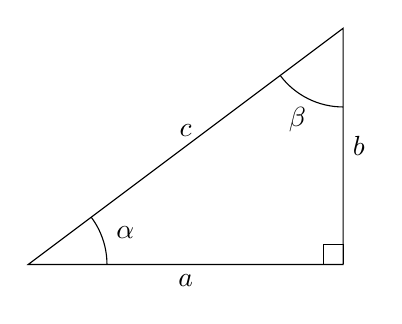
\begin{tikzpicture}
\draw (0,0) coordinate (o);
\draw (4,0) coordinate (u);
\draw (4,3) coordinate (v);
\draw (o)--(u) node[midway, below]{$a$}
--(v) node[midway, right]{$b$}
--(o) node[midway, above]{$c$} --cycle;
\tkzMarkRightAngle(o,u,v);
\tkzMarkAngle(o,v,u);
\tkzLabelAngle[pos=1.3](o,v,u){$\beta$};
\tkzMarkAngle(u,o,v);
\tkzLabelAngle[pos=1.3](u,o,v){$\alpha$};
\end{tikzpicture}

$$
c^2=a^2+b^2
$$
$$
\sin(\alpha)=\frac{b}{c},\quad
\cos(\alpha)=\frac{a}{c},\quad
\tan(\alpha)=\frac{b}{a},\quad
$$
$$
\alpha=\arcsin\frac{b}{c},\quad
=\arccos\frac{b}{c},\quad
=\arctan\frac{b}{c},\quad
$$
$$
\alpha=\textrm{Imag}(\ln(a+bi))\cdot\frac{180^\circ}{\pi}
$$
\end{multicols}

\end{document}